\documentclass[11pt,a4paper]{report}
\usepackage[utf8]{inputenc}
\usepackage[french]{babel}
\usepackage[T1]{fontenc}
\usepackage{amsmath}
\usepackage{amsfonts}
\usepackage{amssymb}
\usepackage{xcolor}
\usepackage{gensymb}

\usepackage{geometry}
\geometry{hmargin=2.5cm,vmargin=1.5cm}
\usepackage{wasysym}
\usepackage{graphicx}

\author{Mathieu Sarrat}
\title{LC20 - Solubilité}

\makeatletter
\renewcommand{\thesection}{\@arabic\c@section}
\makeatother


\begin{document}
\maketitle

\section*{Niveau, Pré-requis et objectifs}
\begin{itemize}
	\item \textbf{Niveau :} MPSI/PTSI\\
	
	\item \textbf{Pré-requis :}
	\begin{itemize}
		\item Constante d'équilibre et activité,
		\item Réactions acido-basiques, d'oxydoréduction, de complexation,
		\item Équivalence lors d'un titrage,
		\item Réaction prépondérante.\\
	\end{itemize}
	
	\item \textbf{Objectifs :}
	\begin{itemize}
		\item Définir la solubilité, la constante de dissolution,
		\item Diagramme d'existence d'un solide,
		\item Applications des réactions de précipitation.\\
	\end{itemize}
		
	\item \textbf{Recommandations :}
	\begin{itemize}
		\item 
	\end{itemize}
	
	\item \textbf{Liste du matériel :}
	\begin{itemize}
		\item Conductimètre et solution d'étalonnage,
		\item Sulfate de calcium solide.\\
	
		\item Gros tube à essais, bec Bunsen et pince en bois,
		\item Solution de nitrate de plomb à 5\%,
		\item Solution d'iodure de potassium à 5\%\\
		
		\item Solution d'acide chlorhydrique à 6 mol/L.\\
		
		\item Sérum physiologique à 0.15 mol/L environ,
		\item Solution de nitrate d'argent à $1.00\times10^{-1}$ mol/L,
		\item Solution de chromate de potassium à 5\%.\\
	\end{itemize} 
\end{itemize}

\newpage
\section*{Introduction}

Lorsqu'on introduit du sel dans l'eau, il se dissout. Si on en met trop, il ne se dissout plus.
\textcolor{blue}{
\begin{itemize}
	\item Faire la manip en direct : la solubilité du sel est de 36g pour 100 mL d'eau  à 				température ambiante.
	\item Bécher 1 : 10 mL d'eau et 1g de sel, ça se dissout.
	\item Bécher 2 : 10 mL d'eau et 5g de sel, ça ne se dissout pas.
	\item Rajouter de l'eau dans le second bécher, ça se dissout.\\
\end{itemize}}
Il doit quelque part exister un seuil en concentration, au-delà duquel il devient impossible de dissoudre un composé solide dans l'eau.\\ 

Jusqu'à présent nous avons étudié exclusivement des réactions en phase homogène (solution aqueuse).Nous allons maintenant nous intéresser à un exemple de réaction en milieu hétérogène (solution aqueuse et précipité solide). Nous allons tout d'abord définir les notions de solubilité, de solution saturée et d'équilibre de solubilité. On expliquera ainsi pourquoi le sel n'est plus soluble dans l'eau au-delà d'une certaine concentration, moment à partir duquel il précipite. Nous mettrons ensuite en évidence divers facteurs agissant sur la solubilité d'un composé, puis détaillerons un certain nombre d'applications des réactions de précipitation au laboratoire et dans la vie quotidienne.

\newpage
\section{Équilibre hétérogène en solution aqueuse}\label{sec:1}

\subsection{Conditions d'existence du solide}

\subsubsection{Constante d'équilibre}
Lorsqu'une espèce est peu soluble dans l'eau, on observe souvent la formation d'un précipité. De même, lorsqu'on essaie de dissoudre une trop grande quantité de solide, il arrive que tout ne se dissolve pas. Il se met en place un \textbf{équilibre hétérogène}, c'est à dire entre deux phases.\\

Lors de la dissolution d'un solide ionique, on obtient les ions constitutifs du solide en solution. Si le solide est moléculaire, on obtient les molécules en solution. Exemples :
\begin{itemize}
	\item dissolution du sulfate de calcium
	\begin{equation}
		\text{CaSO}_{4,\text{(s)}} \rightleftarrows \text{Ca}^{2+} + \text{SO}_4^{2-}, 
		\quad\text{K}_s(T)
	\end{equation}
	\item dissolution du chlorure de plomb
	\begin{equation}
		\text{PbCl}_{2(s)} = {\text{Pb}^{2+}}_\text{(aq)} + 2\;{\text{Cl}^{-}}_\text{(aq)}
	\end{equation}
	\item dissolution du diiode dans l'eau
	\begin{equation}
		\text{I}_{2\text{(s)}} = \text{I}_{2\text{(aq)}}
	\end{equation}
\end{itemize}

\`A tout équilibre chimique est associé une \textbf{constante d'équilibre}, calculée à partir de la loi de Guldberg et Waage en utilisant les activités chimiques des espèces figurant dans l'équation de réaction. Par exemple, dans le cas des équilibres de solubilité du chlorure de plomb et du diiode, on définit
\begin{equation}
	\boxed{\text{K}_s(T) = \left(\frac{[\text{Pb}^{2+}]_\text{eq}}{C\degree}\right)  
	\left(\frac{{[\text{Cl}^-]_\text{eq}}^2}{{C\degree}^2}\right)}
	\quad\text{et}\quad
	\boxed{\text{K}_s(T) = \frac{[\text{I}_2]_\text{eq}}{C\degree}},
\end{equation}
les concentrations étant exprimées en mol/L et $C\degree = 1$ mol/L. L'activité du solide, seul dans sa phase, est pris égale à 1. Cette constante est \textbf{fonction seulement de la température}, et est généralement inférieure à 1. C'est l'analogue d'une constante d'acidité ou d'une constante de formation d'un complexe. Lorsque l'équilibre implique un solide ionique, on parle de \textbf{produit de solubilité}.\\

On définit
\begin{equation}
	\boxed{\text{pK}_s \equiv -\text{log}_{10} \text{K}_s}.
\end{equation}

\subsubsection{Critère d'existence}
Le solide \textbf{doit être présent} pour qu'il y ait équilibre de solubilité. Si le solide est introduit en quantité suffisamment faible, il se dissout totalement et les activités chimiques ne vérifient pas la constante de solubilité.\\

Reprenons l'exemple du sulfate de calcium. En fonction de la valeur du quotient réactionnel $Q_r$ à l'état initial,
\begin{equation}
	\text{Q}_r = [\text{Ca}^{2+}]_0 [{\text{SO}_4}^{2-}]_0
\end{equation}
on en déduit un critère d'existence du solide :\\
\begin{itemize}
	\item si $\text{Q}_r < \text{K}_s(T)$, la solution n'est pas saturée. Les ions ne précipitent 		pas si on les introduit dans l'eau. Si on introduit une quantité de solide telle que les 			concentrations obtenues, s'il se dissout totalement, sont telles que $\text{Q}_r < 
	\text{K}_s(T)$, le solide se dissoudra totalement.
	\item si $\text{Q}_r = \text{K}_s(T)$, il y a équilibre entre le solide et les espèces en 			solution.
	\item si $\text{Q}_r > \text{K}_s(T)$, il y a précipitation jusqu'à ce que la condition 			d'équilibre $\text{Q}_r = \text{K}_s(T)$ soit atteinte.\\
\end{itemize}

\newpage
\subsection{Solubilité dans l'eau pure}
\textcolor{red}{Par conductimétrie : Le Maréchal Chimie Générale, p160}\\

\textbf{Solubilité :} la solubilité d'une espèce solide est la quantité maximale de matière que l'on peut dissoudre dans un litre d'eau. On l'exprime en mol/L ou en g/L (plus fréquent). Lorsqu'une solution est saturée, la quantité de matière passée en solution est déterminée par la solubilité.\\

\textbf{Dissolution du sulfate de calcium dans l'eau :}\\

L'équation de dissolution du solide est la suivante :
\begin{equation}
	\text{CaSO}_{4,\text{(s)}} \rightleftarrows \text{Ca}^{2+} + \text{SO}_4^{2-}, 
	\quad\text{K}_s(T)
\end{equation}
avec
\begin{equation}
	\boxed{\text{K}_s(T) 
	= \frac{[\text{Ca}^{2+}]_\text{eq} [{\text{SO}_4}^{2-}]_\text{eq}}{{C\degree}^2}
	= \frac{s^2}{{\text{C}^0}^2}},
\end{equation}
vérifiée si le solide existe.

\begin{figure}[h!]
	\begin{center}
  		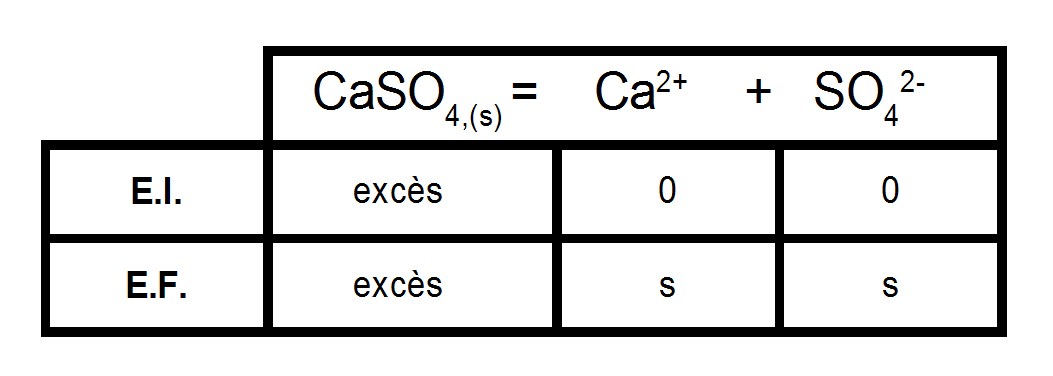
\includegraphics[scale = 0.3]{tableau_avancement.png}
		\caption{Tableau d'avancement de la réaction.}
	\end{center}
\end{figure}

On se propose de mesurer la solubilité du sulfate de calcium dans l'eau et d'en déduire le produit de solubilité $\text{K}_s$ \textcolor{blue}{(relever la température)} à température ambiante. La solubilité du sulfate de calcium dans l'eau est faible, il y aura peu d'ions en solution. On va donc faire la mesure par conductimétrie.\\

\begin{itemize}
	\item \textbf{En préparation :}
	\begin{itemize}
		\item Étalonner le conductimètre
		\item Mesurer la conductance G de l'eau distillée (attention, les concentrations sont 
		en mol/$\text{m}^{-3}$ dans les calculs.
		\item Dans un bécher de 100 mL d'eau distillée, on introduit une spatule de sulfate de 				calcium solide (tout ne doit pas se dissoudre). Introduire un barreau aimanté et agiter. Ne 		pas interrompre l'agitation jusqu'au moment de faire une mesure. On peut aussi filtrer la 			solution pour éliminer le solide.\\
	\end{itemize}
\end{itemize}

\begin{itemize}
	\item \textbf{En direct, mesure et exploitation :}
	\begin{itemize}
		\item Mesurer la conductance G de la solution de sulfate de calcium, retrancher la 						conductance de l'eau distillée.
		\item $\sigma = G L/S$ (avec S/L $=$ 1 cm normalement, pas forcément besoin avec 						étalonnage)\\
		\item \textcolor{blue}{Loi de Kolhrausch :}
		\begin{equation}
			\sigma = \lambda^o(\text{Ca}^{2+})[\text{Ca}^{2+}]_\text{eq} 
			+ \lambda^o({\text{SO}_4}^{2-})[{\text{SO}_4}^{2-}]_\text{eq}
			= \left(\lambda^o(\text{Ca}^{2+}) + \lambda^o({\text{SO}_4}^{2-})\right)\;s,
		\end{equation}
		or les concentrations sont égales, et on connaît les conductivités molaires ioniques limite
		$\lambda^o(\text{Ca}^{2+}) = 11,9\;S.\text{m}^2\text{mol}^{-1}$ 
		et $\lambda^o({\text{SO}_4}^{2-}) = 16.0\;S.\text{m}^2\text{mol}^{-1}$. On remonte à $s$, 			puis à $\text{K}_s = s^2/{C\degree}^2$.
	
		\item La valeur tabulée pour 25\degree C est $K_s = 2.4\times10^{-5}$.	
	\end{itemize}
\end{itemize}

\subsection{Diagramme d'existence et comparaison des $\text{pK}_s$}

\subsubsection{Domaine d'existence du solide}
Soit une solution de nitrate d'argent, à la concentration $\text{C}_0 =$ 0.1 mol/L. Connaissant le $\text{pK}_s$ de l'iodure d'argent ($\text{pK}_s\text{(AgI)} = 15.2$ à 298K), associé à l'équilibre
\begin{equation}
	\text{AgI}_\text{(s)} = {\text{Ag}^+}_\text{(aq)} + {\text{I}^-}_\text{(aq)},
\end{equation}
on veut déterminer à partir de quelle concentration en ions iodure on verra la formation du premier grain de précipité. Lorsque le précipité apparaît, le produit de solubilité est vérifié, donc
\begin{equation}
	[\text{I}^-]_\text{eq} = \frac{K_s}{[\text{Ag}^+]_\text{eq}} = 10^{-14.2}.\\
\end{equation}

En posant 
\begin{equation}
	\text{pI} = -\text{log}_{10} [{\text{I}^-}],\quad\text{on trouve}\quad
	\text{pI}_\text{eq} = 14.2
\end{equation}
au seuil de précipitation.\\

On peut alors représenter un \text{diagramme d'existence} du solide :
\begin{figure}[h!]
	\begin{center}
  		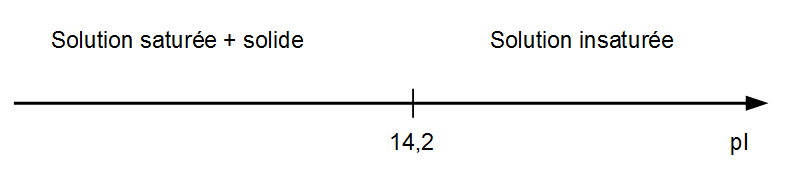
\includegraphics[scale = 0.5]{diagramme_pI.png}
		\caption{Diagramme d'existence du solide.}
	\end{center}
\end{figure}

\textbf{Remarque 1 :} la frontière dépend évidemment de la concentration en l'autre espèce ionique, qui est un choix arbitraire.\\

\textbf{Remarque 2 :} on ne parle pas de diagramme de prédominance, car les espèces ne sont pas présentes dans la même phase, cela n'aurait aucun sens.

\subsubsection{Comparaison des $\text{pK}_s$}

Ne pas croire que l'espèce de $\text{pK}_s$ la plus élevée est la moins soluble. La solubilité dépend aussi de la stœchiométrie de la réaction de dissolution.


\newpage
\section{Paramètres influençant la solubilité}\label{sec:2}

Dans cette partie de la leçon, nous allons mettre en évidence l'influence de plusieurs paramètres sur la solubilité d'une espèce chimique dans l'eau.

\subsection{Influence de la température}
\textcolor{red}{Expérience de la pluie d'or. Le Maréchal, tome 1, p229}\\

Il y a deux effets de la température sur la dissolution d'un solide dans un solvant :\\
\begin{itemize}
	\item \textbf{un effet cinétique} : les corps se dissolvent plus vite dans un solvant chaud que 		dans un solvant froid;
	\item \textbf{un effet thermodynamique} : la constante d'équilibre $\text{K}_s$ dépend de la 			température, et il en va donc de même pour la solubilité $s$.\\
\end{itemize}

\subsubsection{Aspect thermodynamique}
On s'intéresse uniquement à l'aspect thermodynamique de la dissolution :\\
\begin{itemize}
	\item si la dissolution du composé est \textbf{endothermique}, sa solubilité à chaud augmente. 			C'est le cas de l'iodure de plomb, plutôt soluble à chaud et insoluble à froid. 
		\textcolor{blue}{Faire la manip.} La solubilité de l'iodure de plomb est de 0.69 g/L à 				20\degree C et de 4.2 g/L à 100\degree C.\\
		
		Autres exemples, la solubilité du nitrate de potassium (316 g/L à 20\degree C à 1690 g/L
		à 80 \degree C) et celle du chlorure d'ammonium (372 g/L à 20\degree C et 656 g/L 
		à 80 \degree C).\\
		
	\item si la dissolution est \textbf{athermique}, la solubilité varie peu avec la température. 			C'est le cas du chlorure de sodium (on passe de 360 g/L à 358 g/L entre 20 et 80 
		\degree C.\\
	
	\item si la dissolution est \textbf{exothermique}, la solubilité diminue avec la température. 			C'est par exemple le cas de l'hydroxyde de calcium, dont la solubilité passe de 1.65 g/L à 			0.94 g/L entre 20 et 80\degree C.\\
\end{itemize}

\subsubsection{Application à la recristallisation}
Avec l'iodure de plomb, nous avons mis en œuvre une recristallisation : on part d'une poudre et on obtient des cristaux après le refroidissement. Ce procédé de recristallisation peut aussi être utilisé pour purifier un produit de synthèse solide, en jouant sur les différences de solubilité à chaud et à froid du produit à isoler et des impuretés.\\

Lors d'une recristallisation le produit solide, sous forme de poudre, est lavé avant d'être remis en solution ce qui élimine les impuretés très solubles. Ensuite, on chauffe dans une quantité de solvant minimaliste et on filtre pour éliminer les impuretés insolubles à chaud. On refroidit alors lentement : de nombreuses impuretés présentes en solution ne co-précipitent pas (car elles ne sont pas suffisamment concentrées). On peut les éliminer par filtration à froid. En effet, lors d'une cristallisation lente, les ions s'assemblent en respectant des positions minimisant l'énergie, ce qui forme un beau cristal. Si la cristallisation est trop rapide, des impuretés se retrouvent piégées au sein de cristaux mal formés.

\newpage
\subsection{Effet d'ion commun}
\textcolor{blue}{Manip : prélever 1 mL de solution saturée en chlorure de sodium (bécher de la manip d'introduction) et verser le contenu dans 10 mL de solution d'acide chlorhydrique concentrée (au moins 5 mol/L). Un précipité de chlorure de sodium apparaît}.

\subsubsection{Dans l'eau pure}

Le produit de solubilité à 25\degree C du chlorure de sodium est
\begin{equation}
	\text{K}_s = 32.98
\end{equation}
d'où la solubilité du chlorure de sodium dans l'eau pure 
\begin{equation}
	s = 5.74\;\text{mol/L, soit}\quad s = 335\;\text{g/L} \quad\text{et donc}\quad
	s = 3.35\;\text{g pour 10 mL}
\end{equation}
où on a utilisé M(NaCl) $=$ 58,44 g/mol. Le gramme de sel introduit en début de leçon dans 10 mL d'eau distillée est donc totalement dissout. On en déduit le produit de solubilité à 20\degree C.

\subsubsection{Dans la solution de chlorure de potassium}

Quelle est sa valeur dans la solution de chlorure de potassium ? On dresse un tableau d'avancement volumique. On a prélevé 1 mL de solution saturée, soit $\text{n}(\text{Cl}^-) = 5.74\times 10^{-3}$ mol. Ils s'ajoutent aux $6\times 10^{-2}$ mol présents dans les 10 mL de solution de chlorure de potassium. On en déduit la concentration initiale 
\begin{equation}
	\text{C}_0 = \frac{5.74\times 10^{-3} + 6\times 10^{-2}}{11\times 10^{-3}} = 5.98\;\text{mol/L}
\end{equation}

\begin{figure}[h!]
	\begin{center}
  		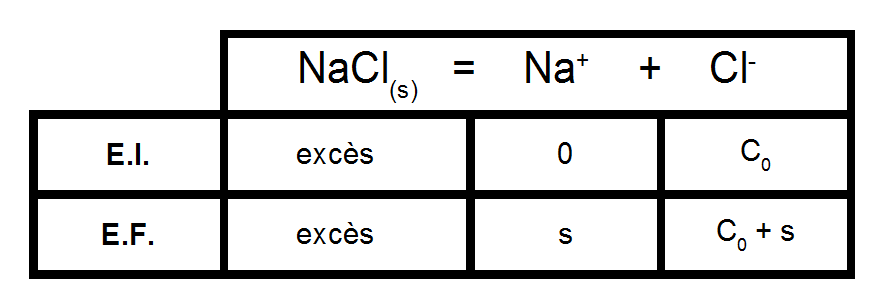
\includegraphics[scale = 0.5]{ion_commun.png}
		\caption{Dissolution du chlorure de sodium dans la solution de chlorure de potassium.}
	\end{center}
\end{figure}

Ainsi, à l'équilibre et sous une température de 25\degree C (la constante conserve sa valeur)
\begin{equation}
	\text{K}\degree (T) = s(\text{C}_0 + s),
\end{equation}
en omettant de faire apparaître les concentrations standard, d'où la valeur de s 
\begin{equation}
	s = 3.48\;\text{mol/L, soit} s = 203.4 g/L
\end{equation}
d'où 2.034 g pour 10 mL, largement inférieur à la solubilité dans l'eau pure.\\

La solubilité du chlorure de sodium diminue fortement dans une solution contenant initialement des ions chlorure. Il en serait de même dans une solution contenant initialement des ions argent.

\newpage
\subsection{Influence de la complexation}

La possibilité de complexation de l'une des espèces dissoutes intervenant dans l'équilibre de solubilité permet d'accroître la solubilité du solide. \textcolor{blue}{Manip de démonstration : former un précipité de chlorure d'argent, ajouter de l'ammoniac concentré en large excès, constater la disparition du précipité blanc.} 

\subsubsection*{Solubilité du chlorure d'argent dans l'eau} 

On donne pKs(AgCl) $=$ 9.75, d'où $K_s(\text{AgCl}) = 10^{-9.75}$, d'où
\begin{equation}
	s = \sqrt{K_s(\text{AgCl})} = \sqrt{[\text{Ag}^+]_\text{eq}[\text{Cl}^-]_\text{eq}}
	= 1.33\times10^{-5}\;\text{mol/L},
\end{equation}
$s$ étant la concentration en ions argent et chlorure à l'équilibre lorsque le solide existe et
$K_s$ étant la \textbf{constante de dissolution}, constante d'équilibre de la réaction
$\text{AgCl}_\text{(s)} = \text{Ag}^+_\text{(aq)} + \text{Cl}^-_\text{(aq)}$.\\

Cette solubilité est très faible. C'est entre autres pour cela qu'il ne faut pas utiliser d'électrode au calomel saturé dans une solution contenant des ions argent. Les ions argent et chlorure vont précipiter dans le verre fritté, boucher l'électrode et la rendre inopérante. On doit utiliser une autre électrode (par exemple sulfate mercureux) ou, faute de mieux, une allonge de protection.

\subsubsection*{Effet de la complexation sur la solubilité}

Tout comme dans la section précédente, nous sommes confrontés à un problème de déplacement d'équilibre. Deux réactions peuvent se produire :
\begin{itemize}
	\item l'équilibre de solubilité
		\begin{equation}
			\text{AgCl}_\text{(s)} \rightleftarrows \text{Ag}^+ + \text{Cl}^-
		\end{equation}
		de constante $K_s = 10^{-9.7}$ (à 298 K)
		\begin{equation}
			\boxed{K_s(\text{AgCl)} = [\text{Ag}^+]_\text{eq}[\text{Cl}^-]_\text{eq}}
		\end{equation}
	\item l'équilibre de formation du complexe,
		\begin{equation}
			\text{Ag}^+ + 2\text{NH}_3 \rightleftarrows [(\text{Ag(NH)}_3)_2]^+
		\end{equation}
		de constante de formation $\beta = 10^{7.2}$ (à 298 K)
		\begin{equation}
			\boxed{\beta = \frac{[[\text{Ag(NH}_3)_2]^+]_\text{eq}}{[\text{Ag}^+]_\text{eq}
			{[\text{NH}_3]_\text{eq}}^2}}
		\end{equation}
\end{itemize}
\textit{Remarque : on a omis de faire apparaître les concentrations standard, donc on travaille en mol/L.}

La réaction de formation du complexe est la réaction prépondérante. On la suppose quantitative ($\beta = 10^{7.2} \gg 1$. Les ions argent libérés par le solide sont aussitôt consommés par l'ammoniac, ce qui provoque la redissolution progressive du solide. Les ions argent seront peu présents en solution, on peut donc modéliser le processus chimique en sommant les deux équations bilan précédentes :
\begin{equation}
	\boxed{\text{AgCl}_\text{(s)} + 2\;\text{NH}_3 = [\text{Ag(NH}_3)_2]^+ + \text{Cl}^-}
\end{equation} 
de constante d'équilibre $K_T\degree = \beta K_s = 10^{-2.5}$ (à 298 K). Cette constante est faible, mais travailler en large excès d'ammoniac permet de déplacer l'équilibre en faveur des produits.\\

Quelle est la solubilité du chlorure d'argent en milieu ammoniacal (on suppose une solution de concentration 1 mol/L en ammoniac) ? L'équilibre de solubilité est réalisé lorsque le solide existe et que la solution est par conséquent saturée, d'où le tableau d'avancement :

\begin{figure}[h!]
	\begin{center}
  		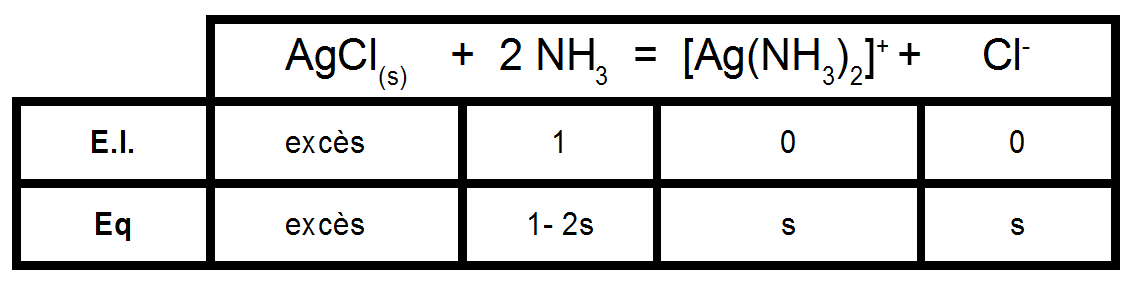
\includegraphics[scale = 0.4]{dissolution_agcl.png}
		\caption{Tableau d'avancement de la réaction de dissolution du chlorure d'argent en milieu 						ammoniacal.}
	\end{center}
\end{figure}

On calcule $s$ à partir de $K_T\degree$, d'où $s = 5.1 \times10^{-2}$ mol/L, soit une valeur bien plus élevée que dans l'eau. On a là un bel exemple de \textbf{loi de modération :} la complexation diminue la concentration en ions argent. Le système réagit pour compenser cette diminution en provoquant la dissolution du solide.

\newpage
\subsection{Influence du pH}

De la même manière, lorsqu'une espèce constituant le précipité présente des propriétés acides ou basiques, la possibilité qu'elle aura de réagir avec d'autres espèces acides ou basiques présentes en solution va jouer sur la solubilité.\\

Prenons l'exemple des carbonates. Le carbonate de calcium $\text{CaCO}_3$(s), plus connu sous le nom de calcaire, est un solide peu soluble dans l'eau : pKs $= 10^{-8.3}$ à 298K. Les ions carbonate ${\text{CO}_3}^{2-}$ sont une base faible, appartenant au couple
\begin{equation}
	{\text{HCO}_3}^-/{\text{CO}_3}^{2-},\quad\text{pK}_{A2} = 10.3
\end{equation}
et l'ion hydrogénocarbonate est une espèce amphotère appartenant au couple
\begin{equation}
	{\text{H}_2\text{CO}_3}/{\text{HCO}_3}^-,\quad\text{pK}_{A1} = 6.4.\\
\end{equation}

Cherchons à exprimer la solubilité $s$ en fonction du pH. Trois réactions sont en jeu :
\begin{equation}
	\text{CaCO}_{3(s)} = \text{Ca}^{2+} + {\text{CO}_3}^{2-}
	\quad\text{de constante d'équilibre}\quad
	K_s = [\text{Ca}^{2+}]_\text{eq}[{\text{CO}_3}^{2-}]_\text{eq}
\end{equation}
\begin{equation}
	{\text{HCO}_3}^- + \text{H}_2\text{O} = \text{H}_3\text{O}^+ + {\text{CO}_3}^{2-}
	\quad\text{de constante d'équilibre}\quad
	K_{A2} = \frac{[{\text{CO}_3}^{2-}]_\text{eq}[\text{H}_3\text{O}^+]_\text{eq}}
	{[{\text{HCO}_3}^-]_\text{eq}}
\end{equation}
\begin{equation}
	{\text{H}_2\text{CO}_3} + \text{H}_2\text{O} = \text{H}_3\text{O}^+ + {\text{HCO}_3}^-
	\quad\text{de constante d'équilibre}\quad
	K_{A1} = \frac{[{\text{HCO}_3}^-]_\text{eq}[\text{H}_3\text{O}^+]_\text{eq}}
	{[{\text{H}_2\text{CO}_3}]_\text{eq}}
\end{equation}

Dans une solution saturée en calcaire, la totalité du solide en solution est sous forme d'ions calcium, d'ions carbonate, hydrogénocarbonate et d'acide carbonique. Ainsi,
\begin{equation}
	s = [\text{Ca}^{2+}] = [{\text{CO}_3}^{2-}] + [{\text{HCO}_3}^-] + [{\text{H}_2\text{CO}_3}]
\end{equation}
\textit{On laisse tomber le eq : les concentrations données sont celles atteintes à l'équilibre}.

On se sert des constantes d'acidité pour exprimer $[{\text{HCO}_3}^-]$ et $[{\text{H}_2\text{CO}_3}]$ avec fonction de $[{\text{CO}_3}^{2-}]$, puis de la constante de solubilité pour remplacer $[{\text{CO}_3}^{2-}]$ :
\begin{equation}
	s = \sqrt{K_s\left(1 + \frac{[\text{H}_3\text{O}^+]}{K_{A2}} + \frac{[\text{H}_3\text{O}^+]^2}{K_{A1}K_{A2}}\right)}
\end{equation}

Il apparaît alors que la solubilité du calcaire dans l'eau augmente lorsque le pH diminue ($[\text{H}_3\text{O}^+]$ augmente). De façon générale, \textbf{on retiendra que la solubilité d'une espèce basique augmente si le pH diminue, alors que celle d'une espèce acide augmente avec le pH.}\\

On peut alors trouver trois expressions approchées en utilisant le diagramme de prédominance des espèces acido-basiques.

\begin{figure}[h!]
	\begin{center}
  		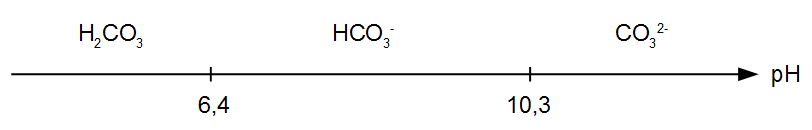
\includegraphics[scale = 0.4]{predo_carbonate.png}
		\caption{Diagramme de prédominance acidobasique de l'acide carbonique.}
	\end{center}
\end{figure}

\begin{itemize}
	\item si pH $> \text{pK}_{A2} + 1 = 11.3 $, l'ion carbonate prédomine et
	\begin{equation}
		s \simeq [{\text{CO}_3}^{2-}] = \frac{K_s}{s} \quad\text{d'où}\quad 
		\text{ps} \equiv -\text{log}\;s = \frac{\text{pKs}}{2} = 4.15;
	\end{equation}
	et l'équilibre de solubilité s'écrit
	\begin{equation}
		\boxed{\text{CaCO}_{3(s)} = \text{Ca}^{2+} + {\text{CO}_3}^{2-}}
	\end{equation}
	\item si $\text{pK}_{A1} + 1 < \text{pH} < \text{pK}_{A2} - 1$
	\begin{equation}
			s \simeq [{\text{HCO}_3}^{-}] 
			\quad\text{d'où}\quad s = \sqrt{\frac{K_s}{K_{A2}}[\text{H}_3\text{O}^+]}
			\quad\text{d'où}\quad \text{ps} \simeq \frac{\text{pH}}{2} - 1
	\end{equation}
	et l'équilibre de solubilité s'écrit
	\begin{equation}
		\text{CaCO}_{3(s)} + \text{H}^+ = \text{Ca}^{2+} + {\text{HCO}_3}^{-} 
	\end{equation}
	On privilégie plutôt l'écriture suivante, le pH étant basique :
	\begin{equation}
		\boxed{\text{CaCO}_{3(s)} + \text{H}_2\text{O} 
		= \text{Ca}^{2+} + {\text{HCO}_3}^{-} + \text{HO}^-}
	\end{equation}
	\item si pH $< \text{pK}_{A1} - 1 = 5.4$
	\begin{equation}
		s \simeq [{\text{H}_2\text{CO}_3}] \quad\text{d'où}\quad 
		\boxed{\text{s} = \sqrt{\frac{K_s}{K_{A2}K_{A1}}}[\text{H}_3\text{O}^+]}
		\quad\text{d'où}\quad \text{ps} = \text{pH} - 4.2
	\end{equation}
	et l'équilibre de solubilité s'écrit
	\begin{equation}
		\boxed{\text{CaCO}_{3(s)} + 2\text{H}^+ = \text{Ca}^{2+} + {\text{H}_2\text{CO}_3}}
	\end{equation}
\end{itemize}

Voilà pourquoi on peut se servir d'une substance acide, comme le vinaigre blanc, pour détartrer une bouilloire. En effet, le tartre est principale composé de calcaire $\text{CaCO}_3$ : on augmente sa solubilité dans l'eau (on le dissout) en le faisant réagir avec de l'acide, en l'occurrence de l'acide acétique. La réaction prépondérante qui aura lieu sera la suivante
\begin{equation}
	{\text{CaCO}_3}_\text{(s)} + 2\;\text{CH}_3\text{COOH}_\text{(aq)} = {\text{Ca}^{2+}}_\text{(aq)} 
	+ {\text{H}_2\text{CO}_3}_\text{(aq)} + 2\;{{\text{CH}_3\text{COO}}^{-}}_\text{(aq)} 
\end{equation}
L'acide carbonique ainsi formé n'est pas stable et se décompose en eau et en gaz carbonique.\\

\section{Applications}

\subsection{Titrage des ions chlorure par la méthode de Mohr}

\subsubsection*{Principe}

Dans trois tubes à essais,
\begin{itemize}
	\item \textbf{Tube 1 :} 1 mL d'une solution incolore de chlorure de sodium à 0,1 mol.$\text{L}^{-1}$ 			et quelques gouttes d'une solution incolore de nitrate d'argent. Il se forme un précipité 					blanc de chlorure d'argent AgCl. Ce précipité est un solide peu soluble dans l'eau :
		\begin{equation}
			\boxed{\text{Ag}^+_\text{(aq)} + \text{Cl}^-_\text{(aq)} = \text{AgCl}_\text{(s)}}
		\end{equation}
		
	\item \textbf{Tube 2 :} 1 mL d’eau distillée, quelques gouttes d'une solution jaune de 
		chromate de potassium $(2\;\text{K}^+_\text{(aq)}+{\text{CrO}_4^{2-}}_\text{(aq)})$,
		quelques gouttes de solution de nitrate d'argent. On observe la formation d'un précipité 					rouge de chromate d'argent $\text{Ag}_2\text{CrO}_4$
		\begin{equation}
			\boxed{2\;\text{Ag}^+_\text{(aq)} + {\text{CrO}_4^{2-}}_\text{(aq)} 
			= \text{Ag}_2\text{CrO}_{4,\text{(s)}}}
		\end{equation}
		
	\item \textbf{Tube 3 :} 1 mL de solution de chlorure de sodium, quelques gouttes de solution de 				chromate de potassium, ajouter \textbf{progressivement} la solution de nitrate d'argent.
		On observe \textbf{d'abord un précipité blanc} de chlorure d'argent (précipité coloré en jaune dû 		aux ions chromate) \textbf{puis un précipité rouge} de chromate d'argent.\\
\end{itemize}
	
\textcolor{blue}{Solubilité du chlorure d'argent :} 
	pKs(AgCl) $=$ 9.75 (à 298 K), d'où $K_s(\text{AgCl}) = 10^{-9.75}$, d'où
\begin{equation}
	s = \sqrt{K_s(\text{AgCl})} = \sqrt{[\text{Ag}^+]_\text{eq}[\text{Cl}^-]_\text{eq}}
	= 1.33\times10^{-5}\;\text{mol/L},
\end{equation}
$s$ étant la concentration en ions argent et chlorure à l'équilibre lorsque le solide existe et
$K_s$ étant la \textbf{constante de dissolution}, constante d'équilibre de la réaction
$\text{AgCl}_\text{(s)} = \text{Ag}^+_\text{(aq)} + \text{Cl}^-_\text{(aq)}$.

\textcolor{blue}{Solubilité du chromate d'argent :} pKs($\text{Ag}_2\text{CrO}_4$) $=$ 11.95 (à 298 K), 
d'où $K_s(\text{Ag}_2\text{CrO}_4) = 10^{-11.95}$. Donc, comme à l'équilibre $[\text{Ag}^+] = 2s$ et $[\text{CrO}_4^{2-}] = s$,
\begin{equation}
	K_s = [\text{Ag}^+]^2[\text{CrO}_4^{2-}] = 4s^3 \quad\text{et donc}\quad s 
	= \left(\frac{K_s}{4}\right)^\frac{1}{3} = 6.54\times10^{-5}\;\text{mol/L}.
\end{equation}

Lorsque deux précipités peuvent se former, c'est le moins soluble dans l'eau qui apparaît en premier \textbf{(phénomène de précipitation préférentielle)}. La solubilité du chlorure d'argent est bien plus faible que celle du chromate d'argent : comme on introduit petit à petit les ions argent, ils vont précipiter préférentiellement avec les ions chlorure plutôt qu'avec les ions chromate.

\subsubsection{Dosage des ions chlorure d'un sérum physiologique (Cachau Redox p404)}

On dose une solution d'ions chlorure $\text{Cl}^-$ de concentration molaire $C_1$ à l'aide d'une solution d'ions $\text{Ag}^+$ de concentration molaire $C_2$ connue, en présence d'une solution de 
\textbf{chromate de potassium servant d'indicateur de fin de réaction} : l'apparition d'un précipité rouge persistant de chromate d'argent marque l'équivalence du dosage. C'est un dosage par titrage direct. \\

\textbf{Matériel :}
\begin{itemize}
	\item Sérum physiologique à $C_1 = 0.15$ mol/L environ;
	\item Solution de nitrate d'argent à $C_2 = 1.00\times10^{-1}$ mol/L;
	\item Solution de chromate de potassium à 5\%.\\
\end{itemize}

\textbf{Protocole :}
Prélever $V_1 =$ 10,00 mL de solution de sérum physiologique (pipette jaugée) de concentration $C_1$ en ion chlorure et les introduire dans un bécher. Ajouter deux gouttes de solution de chromate de potassium à 5\%. On titre par une solution de nitrate d'argent de concentration $C_2 = 1.00\times10^{-1}\;\text{mol}.\text{L}^{-1}$.\\

\textbf{On peut vérifier que le précipité de chlorure d'argent} apparaît dès la première goutte de réactif titrant versée. La première particule de précipité apparaît lorsque le produit de solubilité est vérifié, c'est à dire lorsque la concentration en ions argent est égale à la valeur limite
\begin{equation}
	[\text{Ag}^+] = \frac{K_S}{C_1} \simeq 10^{-9}\;\text{mol/L}.
\end{equation}
Or, la première goutte ($V_\text{goutte} = 0.05$ mL) apporte une quantité d'ions argent
\begin{equation}
	n(\text{Ag}^+) = C_2 \times 0.05\times10^{-3} = 5\times10^{-6}\;\text{mol},
\end{equation}
d'où $[\text{Ag}^+] \simeq n(\text{Ag}^+)/V_1 = 5\times10^{-4}$ mol/L, ce qui est bien supérieur à la valeur limite calculée juste au-dessus.\\

\textbf{Exploitation :}
L'équation du titrage s'écrit
\begin{equation}
	\boxed{\text{Ag}^+_\text{(aq)} + \text{Cl}^-_\text{(aq)} = \text{AgCl}_\text{(s)}}.
\end{equation}

\'A l'équivalence
\begin{equation}
	n_i(\text{Ag}^+) = n_i(\text{Cl}^-) \quad\text{d'où}\quad  C_2\;V_\text{eq} = C_1\;V_1
\end{equation} 
où $V_1$ est le volume de solution titrée. Calculer la concentration en ions chlorure et comparer avec l'étiquette.\\ 

\textbf{Remarque :} en utilisant une électrode d'argent et une électrode au sulfate mercureux, on pourrait faire un suivi potentiométrique pour remonter, en appliquant la loi de Nernst, au $K_s$ du chlorure d'argent.

\subsection{Traitement des effluents}

Les métaux lourds sont des éléments métalliques dont la masse volumique dépasse 5 $\text{g}/\text{cm}^3$. Ils sont le plus souvent présents dans l'environnement sous forme de traces : mercure, argent, plomb, cadmium, cuivre, arsenic, nickel, zinc, cobalt, manganèse. Parmi les plus toxiques d'entre eux se trouvent le mercure et le plomb. La toxicité des métaux lourds n'est plus à démontrer. Ils sont de plus, en général, cancérigènes.\\ 

\begin{figure}[h!]
	\begin{center}
		\begin{tabular}{|c|c|}
		\hline
			\textbf{Hydroxyde métallique} & $K_s$ (298 K)\\
		\hline
		 	$\text{Al(OH)}_3$ & $3\times 10^{-34}$\\
		\hline
			$\text{Cd(OH)}_2$ & $4.5\times 10^{-15}$\\
		\hline
		 	$\text{Cu(OH)}_2$ & $4.8\times 10^{-20}$\\
		\hline
		\end{tabular}	
	\end{center}
	\caption{Quelques hydroxydes métalliques et leur pKs.}
\end{figure}

Les ions métalliques sont des cations solubles dans l'eau mais de nombreux \textbf{hydroxydes métalliques sont peu solubles} dans l'eau. Cette caractéristique permet d'éliminer les métaux lourds des eaux usées par adjonction d’hydroxydes (augmentation du pH). Comme nous l'avons vu, la solubilité d'une espèce manifestant des propriétés acido-basiques (les cations métalliques sont pour la plupart des acides de Lewis) dépend du pH. On utilise de la soude ou de la chaux ($\text{Ca(OH)}_2$) pour agir sur le pH.
On doit donc se placer dans des conditions de pH où les précipités d'hydroxydes métalliques se forment, pour pouvoir ensuite les éliminer par décantation.

\section*{Conclusion}

Nous avons vu ce qu'était une réaction de précipitation et défini la solubilité d'une espèce. Nous avons
mis en évidence plusieurs paramètres influençant un équilibre de solubilité et quelques applications de ces réactions. Les équilibres de solubilité sont souvent en concurrence avec des réactions de complexation ou des réactions acido-basique. Les espèces impliquées dans ces équilibres peuvent aussi manifester des propriétés rédox, comme les ions argent et donc être sensibles à un potentiel d'électrode.\\

Dans la prochaine leçon, nous allons introduire un outil qui nous permettra de prendre en compte simultanément et de façon très visuelle l'influence du pH et du potentiel d'électrode E sur l'état d'équilibre d'un milieu réactionnel dans lequel peuvent se produire des réactions de différentes natures : rédox, acido-basiques, précipitation, complexation. Ce sont les diagrammes potentiel-pH (E-pH). Ils sont une généralisation des diagrammes d'existence et de prédominance que nous avons pu introduire dans les leçons précédentes et dans la leçon actuelle.
\end{document}